\documentclass[a4paper,12pt]{article}

\usepackage{fancyhdr}
\usepackage{lastpage}
\usepackage{amsmath}
\usepackage{tikz}
\usepackage{amsfonts}
\usepackage{graphicx}

\newcommand{\V}[1]{\ensuremath{\vec{#1}}}
\newcommand{\F}[2]{\ensuremath{\frac{#1}{#2}}}
\newcommand{\Q}[1]{\newpage \section*{#1}}
\newcommand{\acc}[1]{\overset{..}{#1}}
\newcommand{\vel}[1]{\overset{.}{#1}}
\newcommand{\prt}[2]{\frac{\partial#1}{\partial#2}}
\newcommand{\LP}{\left(}
\newcommand{\RP}{\right)}


\pagestyle{fancy}
\lhead{Samuel Loomis}
\setlength{\headheight}{15pt}
\chead{Classical Mechanics HW 7}
\rhead{15 November 2013}
\lfoot{}
\cfoot{\thepage\ of \pageref{LastPage}}
\rfoot{}

\begin{document}

\section*{Question 1, Thornton \& Marion, 7-24}

Consider a simple plane pendulum consisting of a mass $m$ attached to a string of length $l$. After the pendulum is set into motion, the length of the string is shortened at a constant rate. \[\F{\partial{l}}{\partial{t}}=-\alpha=constant\] The suspension point remains fixed. Compute the Lagrangian and Hamiltonian functions. Compare the Hamiltonian and the total energy, and discuss the conservation of energy for the system.
\\
\begin{figure}
\centering
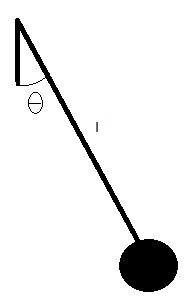
\includegraphics[width=2in]{Pendulum.png}
\end{figure}\\
The position of the pendulum at any point in time is:
\[\V{r}=lsin(\phi)\hat{x}-lcos(\phi)\hat{y}\]
The length $l$ and the angle $\phi$ are both functions of time. Taking the time derivative of $r$ gives:
\[\vel{r}=[\vel{l}sin(\phi)+lcos(\phi)\vel{\phi}]\hat{x}-[\vel{l}cos(\phi)-lsin(\phi)\vel{\phi}]\hat{y}\\\]
The velocity will be used in the kinetic energy, $v^2$:
\begin{align*}
\vel{r}^2=&\vel{l}^2sin^2(\phi)+l^2cos^2(\phi)\vel{\phi}^2+2\vel{l}l\vel{\phi}sin(\phi)cos(\phi)\\
&+\vel{l}^2cos^2{\phi}+l^2sin^2(\phi)\vel{\phi}^2-2\vel{l}l\vel{\phi}sin(\phi)cos(\phi)\\
\vel{r}^2=&\vel{l}^2+l^2\vel{\phi}^2
\end{align*}\\
The kinetic energy $T$ is:
\[T=\F{1}{2}m(\vel{l}^2+l^2\vel{\phi}^2)\]
The potential energy of this system is $mgh$, where $h$ is a time dependent function of $l$ and $\phi$:
\[h=-lcos(\phi)\]
The potential energy $U$ is:
\[U=-mglcos(\phi)\]
The Lagrangian becomes:
\[\mathcal{L}=\F{1}{2}m(\vel{l}^2+l^2\vel{\phi}^2)+mglcos(\phi )\]
The Hamiltonian is equal to:
\[\mathcal{H}=\overset{n}{\underset{i=1}{\Sigma}}p_i\vel{q}_i-\mathcal{L},where~ p_i=\F{\partial\mathcal{L}(q,\vel{q},t)}{\partial\vel{q_i}}\]
As stated earlier, both $l$ and $\phi$ equations vary with time and thus the Hamiltonian needs to be processed with respect to both equation sets.\\
$\vel{l}$:
\[p_l=\prt{\mathcal{L}}{\vel{l}}=m\vel{l}: \vel{l}=\F{p_l}{m}\]
$\vel{\phi}$:
\[p_\phi=\prt{\mathcal{L}}{\vel{\phi}}=2ml^2\vel\phi:\vel\phi=\F{p_\phi}{2ml^2}\]
Writing $\mathcal{H}$ in terms of $p_\phi, p_l, \phi, l$:
\[\mathcal{H}=\F{p_l^2}{m}+\F{p_\phi^2}{2ml^2}-\F{1}{2}m\LP\F{p_l^2}{m^2}+l^2\F{p_\phi^2}{4m^2l^4}\RP+mglcos(\phi)\]
\end{document}


